\documentclass[10pt,aspectratio=169]{beamer}

\usetheme[numbering=fraction,progressbar=foot]{metropolis}

\usepackage[T1]{fontenc}
\usepackage{lmodern}
\usepackage{microtype}
\usepackage{amsmath}
\usepackage{amssymb}
\usepackage{array}
\usepackage{booktabs}
\usepackage{tabularx}
\usepackage{tikz}
\usepackage{graphicx}

\usetikzlibrary{arrows.meta,calc,positioning,shapes.geometric,fit,backgrounds}

\definecolor{Ink}{HTML}{1F2937}
\definecolor{Muted}{HTML}{6B7280}
\definecolor{Sand}{HTML}{F7F4EC}
\definecolor{Paper}{HTML}{FFFDF8}
\definecolor{Mist}{HTML}{E8F1EF}
\definecolor{Peach}{HTML}{F6E4D8}
\definecolor{Slate}{HTML}{DDE4EC}
\definecolor{Gold}{HTML}{C27D38}
\definecolor{Teal}{HTML}{147A73}
\definecolor{Rose}{HTML}{C85C5C}
\definecolor{Night}{HTML}{0F172A}

\setbeamercolor{normal text}{fg=Ink,bg=Sand}
\setbeamercolor{frametitle}{fg=Ink,bg=Sand}
\setbeamercolor{progress bar}{fg=Gold,bg=Slate}
\setbeamercolor{title separator}{fg=Gold}
\setbeamercolor{alerted text}{fg=Gold}
\setbeamercolor{footnote}{fg=Muted}
\setbeamertemplate{navigation symbols}{}
\setbeamersize{text margin left=0.72cm,text margin right=0.72cm}

\title{Music Style Transfer and Genre Remastering}
\subtitle{General Field Overview}
\author{Sahara Kaul \and Kelsey Pattison \and Ahmed Sajid}
\date{CMPUT 414, Winter 2026}

\newcommand{\cardbox}[2]{%
  \begin{tikzpicture}
    \node[
      fill=#1,
      rounded corners=14pt,
      inner xsep=11pt,
      inner ysep=9pt,
      text width=\dimexpr\linewidth-22pt\relax,
      align=left
    ] {\strut #2};
  \end{tikzpicture}%
}

\newcommand{\tagpill}[2]{%
  \tikz[baseline=(x.base)]\node[
    fill=#1,
    rounded corners=7pt,
    inner xsep=7pt,
    inner ysep=3.5pt
  ] (x) {\scriptsize\bfseries #2};%
}

\newcommand{\sectionbanner}[2]{%
  \begin{frame}[plain]
  \begin{tikzpicture}[remember picture,overlay]
    \fill[#1] (current page.south west) rectangle (current page.north east);
    \fill[white,opacity=0.11] ($(current page.north east)+(-0.9,-0.8)$) circle (2.2cm);
    \fill[white,opacity=0.10] ($(current page.south west)+(1.0,0.9)$) circle (1.6cm);
  \end{tikzpicture}
  \vfill
  {\color{white}\usebeamerfont{title}#2\par}
  \vspace{0.22cm}
  {\color{white!82}\Large Music style transfer field overview}
  \vfill
  \end{frame}
}

\newcommand{\refstrip}[1]{{\tiny\color{Muted}#1}}

\begin{document}

\begin{frame}[plain]
\begin{tikzpicture}[remember picture,overlay]
  \fill[Teal!22] ($(current page.south west)+(-0.7,0.4)$) circle (2.9cm);
  \fill[Gold!24] ($(current page.north east)+(-0.9,-0.9)$) circle (2.4cm);
  \fill[Rose!12] ($(current page.north west)+(1.5,-0.7)$) circle (1.3cm);
\end{tikzpicture}

\vspace{0.34cm}
\begin{columns}[T,onlytextwidth]
  \column{0.62\textwidth}
  {\usebeamerfont{title}\color{Ink}\inserttitle\par}
  \vspace{0.2cm}
  {\large\color{Muted}\insertsubtitle\par}
  \vspace{0.48cm}
  {\normalsize\insertauthor\par}
  {\small\color{Muted}\insertdate\par}
  \vspace{0.42cm}
  {\small
    \tagpill{Mist}{Question}
    \hspace{0.35em}
    how do we change style while keeping musical identity recognizable?
  }
  \par\vspace{0.16cm}
  {\small
    \tagpill{Peach}{Theme}
    \hspace{0.35em}
    the field moved from raw generation toward controllable representations
  }
  \par\vspace{0.16cm}
  {\small
    \tagpill{Slate}{Goal}
    \hspace{0.35em}
    explain the concepts first, then the model families that matter most
  }

  \column{0.38\textwidth}
  \cardbox{Paper}{
    \textbf{Speaker split}\\[-0.2em]
    \small
    Kelsey: introduction and concepts\\
    Sarah: early generation, VAEs, MoVE, RAVE\\
    Ahmed: AudioLM, diffusion, and field trends
  }
\end{columns}
\end{frame}

\begin{frame}{Talk Map}
\begin{columns}[T,onlytextwidth]
  \column{0.34\textwidth}
  \cardbox{Peach}{
    \textbf{1. Problem framing}\\[-0.2em]
    \small
    What style transfer means in music, and why it is harder than the image analogy suggests.
  }

  \column{0.33\textwidth}
  \cardbox{Mist}{
    \textbf{2. Early field history}\\[-0.2em]
    \small
    WaveNet, GANs, WaveGAN, GANSynth, and the limits of early audio generation.
  }

  \column{0.33\textwidth}
  \cardbox{Paper}{
    \textbf{3. Modern direction}\\[-0.2em]
    \small
    latent audio, RAVE, AudioLM, diffusion, and why control now matters more than raw novelty
  }
\end{columns}

\vspace{0.28cm}
\begin{center}
\cardbox{Slate}{
  \textbf{Organizing question}\\[-0.2em]
  \small
  Every section should answer: \emph{how does this help preserve content while changing style?}
}
\end{center}
\end{frame}

\sectionbanner{Night}{Part I\\Framing the Problem}

\begin{frame}{What Is Style Transfer?}
\begin{columns}[T,onlytextwidth]
  \column{0.54\textwidth}
  \cardbox{Peach}{
    \textbf{Image analogy}\\[-0.2em]
    \small
    Content is the object layout and scene structure. Style is the color palette, texture, and brush-stroke pattern.
  }
  \vspace{0.16cm}
  \cardbox{Mist}{
    \textbf{Music version}\\[-0.2em]
    \small
    Instead of changing color, we want to change timbre, instrumentation, texture, articulation, and production character.
  }

  \column{0.46\textwidth}
  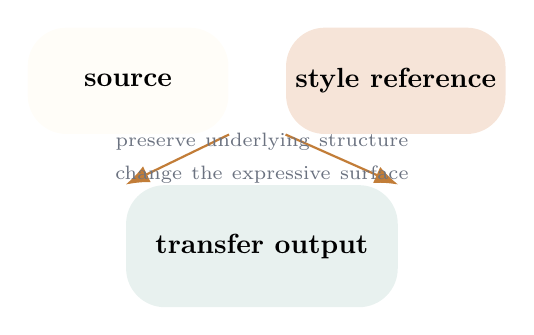
\begin{tikzpicture}[>=Latex]
    \node[fill=Paper, rounded corners=14pt, minimum width=2.55cm, minimum height=1.35cm] (a) at (1.4,3.1) {\textbf{source}};
    \node[fill=Peach, rounded corners=14pt, minimum width=2.75cm, minimum height=1.35cm] (b) at (4.8,3.1) {\textbf{style reference}};
    \node[fill=Mist, rounded corners=14pt, minimum width=3.45cm, minimum height=1.55cm] (c) at (3.1,1.0) {\textbf{transfer output}};
    \draw[-{Latex[length=3mm]}, thick, color=Gold] (a.south east) -- (c.north west);
    \draw[-{Latex[length=3mm]}, thick, color=Gold] (b.south west) -- (c.north east);
    \node[align=center, text width=3.9cm, color=Muted] at (3.1,2.12) {\scriptsize preserve underlying structure\\change the expressive surface};
  \end{tikzpicture}
\end{columns}
\end{frame}

\begin{frame}{Style Versus Content}
\begin{columns}[T,onlytextwidth]
  \column{0.48\textwidth}
  \cardbox{Peach}{
    \textbf{Content}\\[-0.2em]
    \small
    \begin{itemize}
      \item melody
      \item rhythm
      \item notes being played
      \item broad harmonic path
      \item phrase contour
    \end{itemize}
  }

  \column{0.48\textwidth}
  \cardbox{Mist}{
    \textbf{Style}\\[-0.2em]
    \small
    \begin{itemize}
      \item timbre and tone quality
      \item instrumentation
      \item texture and density
      \item dynamics and articulation
      \item expressive details
    \end{itemize}
  }
\end{columns}

\vspace{0.18cm}
\begin{equation*}
x_{\mathrm{src}} \rightarrow \hat{x}_{\mathrm{tgt}}
\qquad \text{with} \qquad
\mathrm{content}(\hat{x}_{\mathrm{tgt}}) \approx \mathrm{content}(x_{\mathrm{src}})
\end{equation*}
\end{frame}

\begin{frame}{Why Music Style Transfer Is Harder Than It First Seems}
\begin{columns}[T,onlytextwidth]
  \column{0.5\textwidth}
  \cardbox{Paper}{
    \textbf{Music is multilevel}\\[-0.2em]
    \small
    Melody, rhythm, harmony, texture, instrumentation, room acoustics, mixing, and long-range form all live in the same signal.
  }
  \vspace{0.16cm}
  \cardbox{Peach}{
    \textbf{Entanglement problem}\\[-0.2em]
    \small
    Changing one layer often damages another. A timbre edit can distort melody, phrase identity, or realism.
  }

  \column{0.5\textwidth}
  \cardbox{Mist}{
    \textbf{The coat-of-paint failure mode}\\[-0.2em]
    \small
    Weak systems sound processed rather than genuinely re-authored. The arrangement still feels like the source.
  }
  \vspace{0.16cm}
  \cardbox{Slate}{
    \textbf{Genre makes this harder}\\[-0.2em]
    \small
    Genre is not one surface sound. It is a broader manifold shaped by groove, conventions, production norms, and listener expectations.
  }
\end{columns}
\end{frame}

\begin{frame}{Musical Representations}
\begin{columns}[T,onlytextwidth]
  \column{0.56\textwidth}
  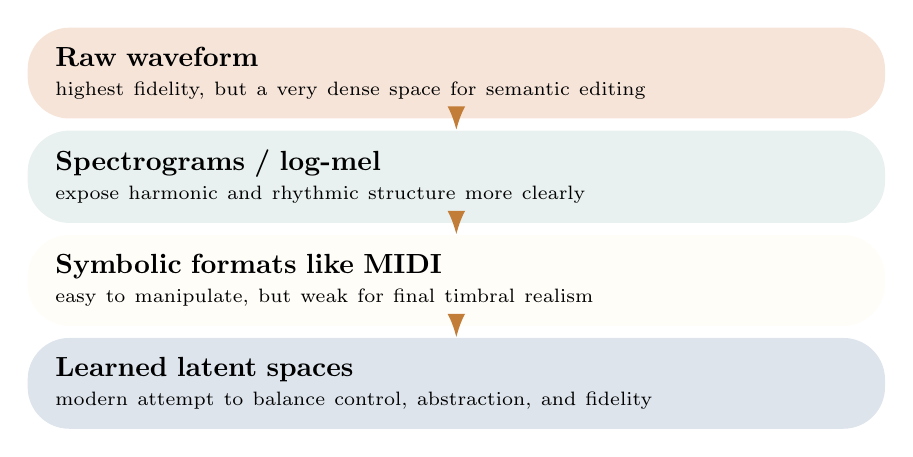
\begin{tikzpicture}[>=Latex, node distance=0.14cm]
    \node[fill=Peach, rounded corners=15pt, text width=0.84\linewidth, inner xsep=10pt, inner ysep=7pt] (a) {
      \textbf{Raw waveform}\\[-0.15em]
      \scriptsize highest fidelity, but a very dense space for semantic editing
    };
    \node[fill=Mist, rounded corners=15pt, text width=0.84\linewidth, inner xsep=10pt, inner ysep=7pt, below=of a] (b) {
      \textbf{Spectrograms / log-mel}\\[-0.15em]
      \scriptsize expose harmonic and rhythmic structure more clearly
    };
    \node[fill=Paper, rounded corners=15pt, text width=0.84\linewidth, inner xsep=10pt, inner ysep=7pt, below=of b] (c) {
      \textbf{Symbolic formats like MIDI}\\[-0.15em]
      \scriptsize easy to manipulate, but weak for final timbral realism
    };
    \node[fill=Slate, rounded corners=15pt, text width=0.84\linewidth, inner xsep=10pt, inner ysep=7pt, below=of c] (d) {
      \textbf{Learned latent spaces}\\[-0.15em]
      \scriptsize modern attempt to balance control, abstraction, and fidelity
    };
    \draw[-{Latex[length=3mm]}, thick, color=Gold] (a.south) -- (b.north);
    \draw[-{Latex[length=3mm]}, thick, color=Gold] (b.south) -- (c.north);
    \draw[-{Latex[length=3mm]}, thick, color=Gold] (c.south) -- (d.north);
  \end{tikzpicture}

  \column{0.44\textwidth}
  \cardbox{Paper}{
    \textbf{Recurring field lesson}\\[-0.2em]
    \small
    Representation choice often matters as much as architecture choice.
  }
  \vspace{0.16cm}
  \cardbox{Mist}{
    \textbf{Practical implication}\\[-0.2em]
    \small
    Many important model advances are really advances in \emph{where} generation happens.
  }
\end{columns}
\end{frame}

\begin{frame}{STFT and MIDI: Two Useful Anchors}
\begin{columns}[T,onlytextwidth]
  \column{0.5\textwidth}
  \cardbox{Peach}{
    \textbf{Fourier Transform and STFT}\\[-0.2em]
    \small
    The Fourier Transform tells us which frequencies are present overall. The STFT applies it to short overlapping windows, giving a time-frequency picture of the sound.
  }
  \vspace{0.16cm}
  \begin{equation*}
    X(m,\omega)=\sum_n x[n]\,w[n-m]\,e^{-j\omega n}
  \end{equation*}

  \column{0.5\textwidth}
  \cardbox{Mist}{
    \textbf{MIDI versus audio}\\[-0.2em]
    \small
    MIDI stores musical events such as note onsets, durations, and velocities. It is compact and editable, but it does not directly capture final timbre or production character.
  }
  \vspace{0.16cm}
  \cardbox{Paper}{
    \textbf{Why this matters}\\[-0.2em]
    \small
    Symbolic generation is easier, but audio style transfer needs waveform realism and sonic detail.
  }
\end{columns}
\end{frame}

\begin{frame}{Core Challenges in Music Style Transfer}
\begin{columns}[T,onlytextwidth]
  \column{0.5\textwidth}
  \cardbox{Peach}{
    \textbf{Representation problem}\\[-0.2em]
    \small
    what is the right working space for controllable editing?
  }
  \vspace{0.16cm}
  \cardbox{Mist}{
    \textbf{Disentanglement problem}\\[-0.2em]
    \small
    how can content be preserved while style is changed?
  }

  \column{0.5\textwidth}
  \cardbox{Paper}{
    \textbf{Realism problem}\\[-0.2em]
    \small
    even a structurally correct output fails if it sounds phasey, noisy, or synthetic
  }
  \vspace{0.16cm}
  \cardbox{Slate}{
    \textbf{Long-form coherence problem}\\[-0.2em]
    \small
    local quality is not enough if longer outputs drift or break at chunk boundaries
  }
\end{columns}

\vspace{0.18cm}
\begin{center}
\cardbox{Paper}{
  \textbf{Field structure}\\[-0.2em]
  \small
  Early models struggled with representation and realism. Later work focused on disentanglement, latent controllability, and re-authoring.
}
\end{center}
\end{frame}

\sectionbanner{Night}{Part II\\Early Audio Generation and Latent Audio}

\begin{frame}{WaveNet}
\begin{columns}[T,onlytextwidth]
  \column{0.52\textwidth}
  \cardbox{Peach}{
    \textbf{What it was}\\[-0.2em]
    \small
    One of the first major neural systems to generate realistic audio with autoregressive sample-by-sample prediction.
  }
  \vspace{0.16cm}
  \cardbox{Mist}{
    \textbf{Core mechanism}\\[-0.2em]
    \small
    dilated causal convolutions let the model see larger temporal context without looking into the future
  }

  \column{0.48\textwidth}
  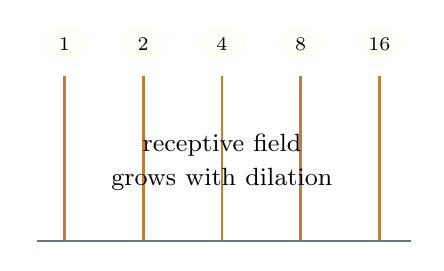
\begin{tikzpicture}[>=Latex]
    \foreach \x/\lab in {0.8/1,1.8/2,2.8/4,3.8/8,4.8/16} {
      \draw[color=Gold, line width=1pt] (\x,0.7) -- (\x,2.8);
      \node[fill=Paper, rounded corners=8pt, minimum width=0.65cm, minimum height=0.42cm] at (\x,3.2) {\scriptsize \lab};
    }
    \draw[thick,color=Muted] (0.45,0.7) -- (5.2,0.7);
    \node[align=center,text width=4.7cm] at (2.8,1.7) {\small receptive field grows with dilation};
  \end{tikzpicture}
  \vspace{0.12cm}
  \cardbox{Paper}{
    \textbf{Why it is only background}\\[-0.2em]
    \small
    It showed that high-quality neural audio was possible, but it was slow and not a practical direct answer to style transfer.
  }
\end{columns}
\end{frame}

\begin{frame}{Background About GANs}
\begin{columns}[T,onlytextwidth]
  \column{0.52\textwidth}
  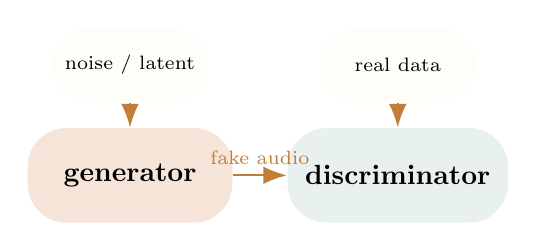
\begin{tikzpicture}[>=Latex]
    \node[fill=Peach, rounded corners=14pt, minimum width=2.6cm, minimum height=1.2cm] (g) at (1.8,2.1) {\textbf{generator}};
    \node[fill=Mist, rounded corners=14pt, minimum width=2.8cm, minimum height=1.2cm] (d) at (5.2,2.1) {\textbf{discriminator}};
    \node[fill=Paper, rounded corners=14pt, minimum width=2.0cm, minimum height=0.95cm] (z) at (1.8,3.5) {\scriptsize noise / latent};
    \node[fill=Paper, rounded corners=14pt, minimum width=2.0cm, minimum height=0.95cm] (r) at (5.2,3.5) {\scriptsize real data};
    \draw[-{Latex[length=3mm]}, thick, color=Gold] (z.south) -- (g.north);
    \draw[-{Latex[length=3mm]}, thick, color=Gold] (g.east) -- node[above,sloped] {\scriptsize fake audio} (d.west);
    \draw[-{Latex[length=3mm]}, thick, color=Gold] (r.south) -- (d.north);
  \end{tikzpicture}

  \column{0.48\textwidth}
  \cardbox{Peach}{
    \textbf{Generator}\\[-0.2em]
    \small
    produces candidate samples from noise or latent codes
  }
  \vspace{0.16cm}
  \cardbox{Mist}{
    \textbf{Discriminator}\\[-0.2em]
    \small
    learns to distinguish real from fake and pushes the generator toward realism
  }
  \vspace{0.16cm}
  \cardbox{Paper}{
    \textbf{Historical role}\\[-0.2em]
    \small
    GANs often produced sharper outputs than plain autoencoders, but stability remained difficult.
  }
\end{columns}
\end{frame}

\begin{frame}{WaveGAN}
\begin{columns}[T,onlytextwidth]
  \column{0.52\textwidth}
  \cardbox{Peach}{
    \textbf{Key idea}\\[-0.2em]
    \small
    Adapt image GAN ideas to one-dimensional audio by using 1D convolutions, larger stride, and no batch normalization.
  }
  \vspace{0.16cm}
  \cardbox{Mist}{
    \textbf{Phase shuffle}\\[-0.2em]
    \small
    random phase shifts stop the discriminator from relying too heavily on trivial phase artifacts
  }

  \column{0.48\textwidth}
  \cardbox{Paper}{
    \textbf{What it showed}\\[-0.2em]
    \small
    parallel raw-audio generation was possible
  }
  \vspace{0.16cm}
  \cardbox{Slate}{
    \textbf{Two major limits}\\[-0.2em]
    \small
    \begin{itemize}
      \item phase precession made outputs sound phasey or unnatural
      \item fixed short clips made long-form coherent generation difficult
    \end{itemize}
  }
\end{columns}
\end{frame}

\begin{frame}{GANSynth}
\begin{columns}[T,onlytextwidth]
  \column{0.55\textwidth}
  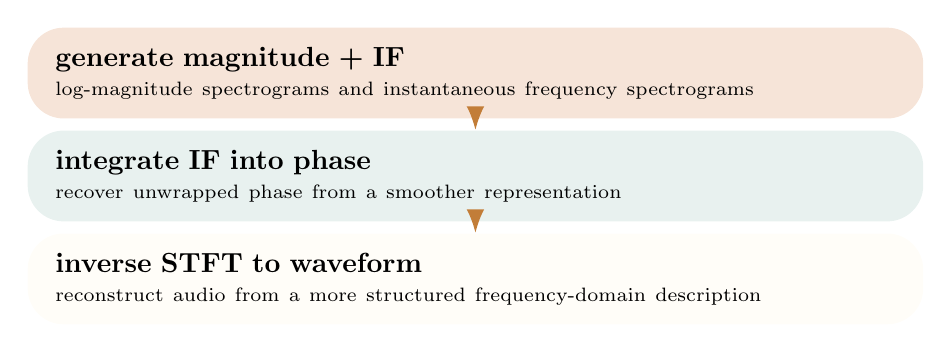
\begin{tikzpicture}[>=Latex, node distance=0.14cm]
    \node[fill=Peach, rounded corners=13pt, text width=0.88\linewidth, inner xsep=10pt, inner ysep=7pt] (a) {
      \textbf{generate magnitude + IF}\\[-0.15em]
      \scriptsize log-magnitude spectrograms and instantaneous frequency spectrograms
    };
    \node[fill=Mist, rounded corners=13pt, text width=0.88\linewidth, inner xsep=10pt, inner ysep=7pt, below=of a] (b) {
      \textbf{integrate IF into phase}\\[-0.15em]
      \scriptsize recover unwrapped phase from a smoother representation
    };
    \node[fill=Paper, rounded corners=13pt, text width=0.88\linewidth, inner xsep=10pt, inner ysep=7pt, below=of b] (c) {
      \textbf{inverse STFT to waveform}\\[-0.15em]
      \scriptsize reconstruct audio from a more structured frequency-domain description
    };
    \draw[-{Latex[length=3mm]}, thick, color=Gold] (a.south) -- (b.north);
    \draw[-{Latex[length=3mm]}, thick, color=Gold] (b.south) -- (c.north);
  \end{tikzpicture}

  \column{0.45\textwidth}
  \cardbox{Mist}{
    \textbf{Why it helped}\\[-0.2em]
    \small
    Instantaneous frequency is more stable than raw phase, so the model avoids some of WaveGAN's phase problems.
  }
  \vspace{0.16cm}
  \cardbox{Paper}{
    \textbf{Field lesson}\\[-0.2em]
    \small
    Representation choice matters. A better working space can improve realism more than brute-force raw waveform generation.
  }
\end{columns}
\end{frame}

\begin{frame}{Why Early Audio Generation Was Not Enough}
\begin{columns}[T,onlytextwidth]
  \column{0.5\textwidth}
  \cardbox{Peach}{
    \textbf{WaveNet, WaveGAN, GANSynth}\\[-0.2em]
    \small
    all helped prove that neural audio generation was possible
  }
  \vspace{0.16cm}
  \cardbox{Mist}{
    \textbf{But they stayed weak for transfer}\\[-0.2em]
    \small
    they could generate or condition audio, but did not explicitly guarantee content preservation
  }

  \column{0.5\textwidth}
  \cardbox{Paper}{
    \textbf{Three combined takeaways}\\[-0.2em]
    \small
    \begin{enumerate}
      \item raw audio generation was possible
      \item representation choice matters
      \item preserving content while changing style remained unsolved
    \end{enumerate}
  }
\end{columns}
\end{frame}

\begin{frame}{VAEs and Latent Audio}
\begin{columns}[T,onlytextwidth]
  \column{0.55\textwidth}
  \begin{equation*}
    x \xrightarrow{\text{encoder}} z \xrightarrow{\text{decoder}} \hat{x}
  \end{equation*}
  \cardbox{Peach}{
    \textbf{Why VAEs were attractive}\\[-0.2em]
    \small
    A latent space gives a structured place where musical properties might be manipulated.
  }

  \column{0.45\textwidth}
  \cardbox{Mist}{
    \textbf{Why naive VAEs struggled on raw audio}\\[-0.2em]
    \small
    \begin{itemize}
      \item posterior collapse
      \item one weak global bottleneck
      \item sequential reconstruction difficulty
    \end{itemize}
  }
  \vspace{0.16cm}
  \cardbox{Paper}{
    \textbf{Still important}\\[-0.2em]
    \small
    The latent-space idea remained valuable even when the first audio VAEs were weak.
  }
\end{columns}
\end{frame}

\begin{frame}{MoVE}
\begin{columns}[T,onlytextwidth]
  \column{0.54\textwidth}
  \cardbox{Peach}{
    \textbf{What MoVE is}\\[-0.2em]
    \small
    Modulated Variational auto-Encoders for many-to-many musical timbre transfer
  }
  \vspace{0.16cm}
  \cardbox{Mist}{
    \textbf{Why it matters}\\[-0.2em]
    \small
    It was built specifically for musical timbre transfer, not just generic audio generation.
  }

  \column{0.46\textwidth}
  \cardbox{Paper}{
    \textbf{Main ingredients}\\[-0.2em]
    \small
    \begin{itemize}
      \item VAE latent structure
      \item FiLM conditioning
      \item many-to-many transfer in one multi-domain model
      \item MMD objective to align distributions
    \end{itemize}
  }
  \vspace{0.16cm}
  \cardbox{Slate}{
    \textbf{Limitation}\\[-0.2em]
    \small
    mainly timbre transfer rather than full genre remastering
  }
\end{columns}
\end{frame}

\begin{frame}{RAVE}
\begin{columns}[T,onlytextwidth]
  \column{0.55\textwidth}
  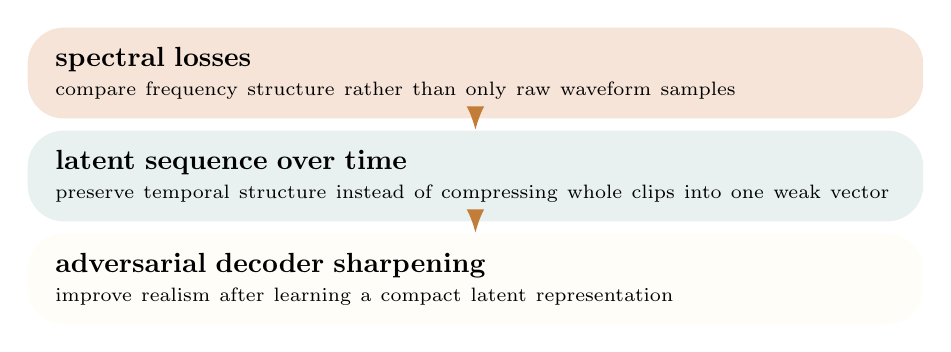
\begin{tikzpicture}[>=Latex, node distance=0.14cm]
    \node[fill=Peach, rounded corners=13pt, text width=0.88\linewidth, inner xsep=10pt, inner ysep=7pt] (a) {
      \textbf{spectral losses}\\[-0.15em]
      \scriptsize compare frequency structure rather than only raw waveform samples
    };
    \node[fill=Mist, rounded corners=13pt, text width=0.88\linewidth, inner xsep=10pt, inner ysep=7pt, below=of a] (b) {
      \textbf{latent sequence over time}\\[-0.15em]
      \scriptsize preserve temporal structure instead of compressing whole clips into one weak vector
    };
    \node[fill=Paper, rounded corners=13pt, text width=0.88\linewidth, inner xsep=10pt, inner ysep=7pt, below=of b] (c) {
      \textbf{adversarial decoder sharpening}\\[-0.15em]
      \scriptsize improve realism after learning a compact latent representation
    };
    \draw[-{Latex[length=3mm]}, thick, color=Gold] (a.south) -- (b.north);
    \draw[-{Latex[length=3mm]}, thick, color=Gold] (b.south) -- (c.north);
  \end{tikzpicture}

  \column{0.45\textwidth}
  \cardbox{Mist}{
    \textbf{Why RAVE matters for style transfer}\\[-0.2em]
    \small
    It made high-quality latent audio practical, which made editing and transfer much more realistic.
  }
  \vspace{0.16cm}
  \cardbox{Paper}{
    \textbf{Position in the story}\\[-0.2em]
    \small
    RAVE is a major step from generic latent modeling toward controllable neural audio.
  }
\end{columns}

\vspace{0.06cm}
\refstrip{RAVE: Caillon and Esling (2021).}
\end{frame}

\sectionbanner{Night}{Part III\\Modern Controllable Synthesis}

\begin{frame}{AudioLM and Long-Range Structure}
\begin{columns}[T,onlytextwidth]
  \column{0.55\textwidth}
  \cardbox{Peach}{
    \textbf{What AudioLM does}\\[-0.2em]
    \small
    Treat audio generation like language modeling over discrete tokens.
  }
  \vspace{0.16cm}
  \cardbox{Mist}{
    \textbf{Important idea}\\[-0.2em]
    \small
    Separate token streams for long-range structure and fine acoustic detail.
  }

  \column{0.45\textwidth}
  \cardbox{Paper}{
    \textbf{Why it matters here}\\[-0.2em]
    \small
    It is not a style-transfer model directly, but it addresses one of the hardest downstream problems: long-form coherence.
  }
  \vspace{0.16cm}
  \cardbox{Slate}{
    \textbf{Field role}\\[-0.2em]
    \small
    evidence that modern audio models can preserve meaningful structure over longer spans
  }
\end{columns}
\end{frame}

\begin{frame}{BigVGAN and FiLM}
\begin{columns}[T,onlytextwidth]
  \column{0.5\textwidth}
  \cardbox{Peach}{
    \textbf{BigVGAN}\\[-0.2em]
    \small
    A universal neural vocoder that turns intermediate representations such as mel-spectrograms into more realistic waveform audio.
  }
  \vspace{0.16cm}
  \begin{equation*}
    f(x)=x+\frac{1}{\alpha}\sin^2(\alpha x)
  \end{equation*}
  \vspace{-0.12cm}
  \cardbox{Paper}{
    \textbf{Role}\\[-0.2em]
    \small
    realism stage rather than transfer logic
  }

  \column{0.5\textwidth}
  \cardbox{Mist}{
    \textbf{FiLM}\\[-0.2em]
    \small
    Feature-wise Linear Modulation lets a condition vector scale and shift hidden features throughout a network.
  }
  \vspace{0.16cm}
  \begin{equation*}
    \mathrm{FiLM}(F;c)=\gamma(c)\odot F+\beta(c)
  \end{equation*}
  \vspace{-0.12cm}
  \cardbox{Slate}{
    \textbf{Role}\\[-0.2em]
    \small
    directly relevant to style-control logic
  }
\end{columns}
\end{frame}

\begin{frame}{DDPM}
\begin{columns}[T,onlytextwidth]
  \column{0.56\textwidth}
  \begin{equation*}
    q(x_t\mid x_0)=\mathcal{N}\!\left(\sqrt{\bar{\alpha}_t}x_0,\,(1-\bar{\alpha}_t)I\right)
  \end{equation*}
  \cardbox{Peach}{
    \textbf{Core idea}\\[-0.2em]
    \small
    Gradually destroy a sample with noise, then learn the reverse process that reconstructs it.
  }

  \column{0.44\textwidth}
  \cardbox{Mist}{
    \textbf{Why diffusion matters}\\[-0.2em]
    \small
    \begin{itemize}
      \item more stable than adversarial training in many settings
      \item iterative generation gives more room for control
      \item better suited to re-authoring than one-shot synthesis
    \end{itemize}
  }
\end{columns}
\end{frame}

\begin{frame}{Classifier-Free Guidance and SDEdit}
\begin{columns}[T,onlytextwidth]
  \column{0.54\textwidth}
  \begin{equation*}
    \hat{\epsilon}_{\mathrm{cfg}}=
    \epsilon_{\theta}(x_t,t,\varnothing)+
    w\left[\epsilon_{\theta}(x_t,t,c)-\epsilon_{\theta}(x_t,t,\varnothing)\right]
  \end{equation*}
  \vspace{-0.12cm}
  \cardbox{Peach}{
    \textbf{CFG}\\[-0.2em]
    \small
    guidance scale $w$ is a practical knob for how aggressively target style should dominate
  }
  \vspace{0.16cm}
  \begin{equation*}
    x(t)=\alpha(t)x(0)+\sigma(t)z,\qquad z\sim\mathcal{N}(0,I)
  \end{equation*}

  \column{0.46\textwidth}
  \cardbox{Mist}{
    \textbf{SDEdit}\\[-0.2em]
    \small
    start from a noised version of an existing source instead of pure noise
  }
  \vspace{0.16cm}
  \cardbox{Paper}{
    \textbf{Why these matter for style transfer}\\[-0.2em]
    \small
    Together they make the content-versus-style tradeoff explicit rather than implicit.
  }
\end{columns}
\end{frame}

\begin{frame}{AudioLDM and Why Diffusion Is the Modern Direction}
\begin{columns}[T,onlytextwidth]
  \column{0.52\textwidth}
  \cardbox{Peach}{
    \textbf{AudioLDM}\\[-0.2em]
    \small
    Latent diffusion for audio shows that high-quality controllable generation can happen in learned latent spaces rather than directly in waveform space.
  }
  \vspace{0.16cm}
  \cardbox{Mist}{
    \textbf{Why it is relevant}\\[-0.2em]
    \small
    It makes diffusion feel much more applicable to editing and transformation, not only text-to-audio generation.
  }

  \column{0.48\textwidth}
  \cardbox{Paper}{
    \textbf{Why diffusion leads the current story}\\[-0.2em]
    \small
    \begin{itemize}
      \item progressive generation
      \item strong conditioning
      \item explicit guidance control
      \item source anchoring through editing-style formulations
    \end{itemize}
  }
  \vspace{0.16cm}
  \cardbox{Slate}{
    \textbf{Main claim}\\[-0.2em]
    \small
    Diffusion is central not because it is trendy, but because it matches the style-transfer problem better than many earlier families.
  }
\end{columns}
\end{frame}

\begin{frame}{Overview of Field Trends}
\begin{columns}[T,onlytextwidth]
  \column{0.53\textwidth}
  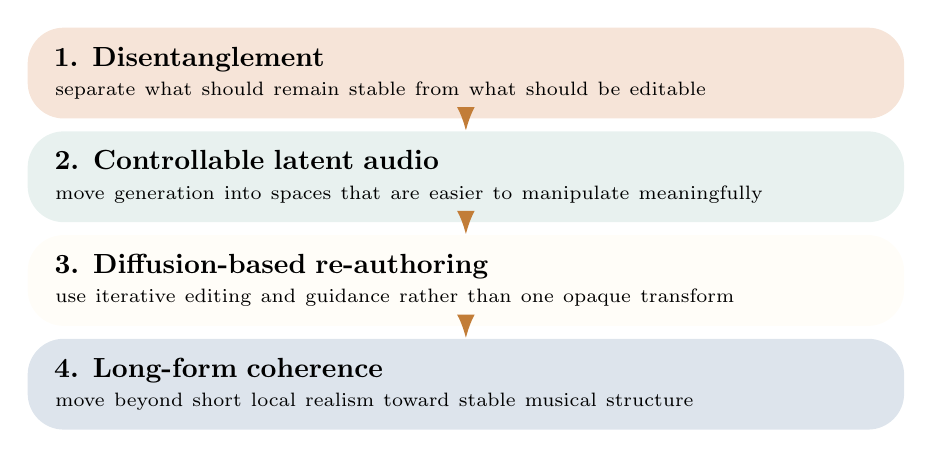
\begin{tikzpicture}[>=Latex, node distance=0.15cm]
    \node[fill=Peach, rounded corners=13pt, text width=0.86\linewidth, inner xsep=10pt, inner ysep=7pt] (a) {
      \textbf{1. Disentanglement}\\[-0.15em]
      \scriptsize separate what should remain stable from what should be editable
    };
    \node[fill=Mist, rounded corners=13pt, text width=0.86\linewidth, inner xsep=10pt, inner ysep=7pt, below=of a] (b) {
      \textbf{2. Controllable latent audio}\\[-0.15em]
      \scriptsize move generation into spaces that are easier to manipulate meaningfully
    };
    \node[fill=Paper, rounded corners=13pt, text width=0.86\linewidth, inner xsep=10pt, inner ysep=7pt, below=of b] (c) {
      \textbf{3. Diffusion-based re-authoring}\\[-0.15em]
      \scriptsize use iterative editing and guidance rather than one opaque transform
    };
    \node[fill=Slate, rounded corners=13pt, text width=0.86\linewidth, inner xsep=10pt, inner ysep=7pt, below=of c] (d) {
      \textbf{4. Long-form coherence}\\[-0.15em]
      \scriptsize move beyond short local realism toward stable musical structure
    };
    \draw[-{Latex[length=3mm]}, thick, color=Gold] (a.south) -- (b.north);
    \draw[-{Latex[length=3mm]}, thick, color=Gold] (b.south) -- (c.north);
    \draw[-{Latex[length=3mm]}, thick, color=Gold] (c.south) -- (d.north);
  \end{tikzpicture}

  \column{0.47\textwidth}
  \cardbox{Paper}{
    \textbf{The larger shift}\\[-0.2em]
    \small
    The field moved from raw generation tricks toward structured representations, explicit control, and longer-horizon musical stability.
  }
  \vspace{0.16cm}
  \cardbox{Mist}{
    \textbf{This is why the emphasis changed}\\[-0.2em]
    \small
    MoVE, RAVE, AudioLM, and AudioLDM now say more about the field than a long walkthrough of older waveform internals.
  }
\end{columns}
\end{frame}

\begin{frame}{Conclusion}
\begin{columns}[T,onlytextwidth]
  \column{0.56\textwidth}
  \cardbox{Peach}{
    \textbf{Main lesson}\\[-0.2em]
    \small
    Music style transfer is not just an audio-generation problem. It is simultaneously a structure-preservation, representation, conditioning, synthesis, and coherence problem.
  }
  \vspace{0.16cm}
  \cardbox{Mist}{
    \textbf{Historical arc}\\[-0.2em]
    \small
    Early waveform models proved that neural audio was possible. Later work made the field more controllable, more structured, and more relevant to real transfer.
  }

  \column{0.44\textwidth}
  \cardbox{Paper}{
    \textbf{Final framing}\\[-0.2em]
    \small
    The field is moving from surface transfer toward structure-aware genre reconstruction.
  }
  \vspace{0.16cm}
  \cardbox{Slate}{
    \textbf{Key models to remember}\\[-0.2em]
    \small
    WaveNet, WaveGAN, GANSynth, MoVE, RAVE, AudioLM, BigVGAN, DDPM, CFG, SDEdit, AudioLDM
  }
\end{columns}
\end{frame}

\end{document}
